\documentclass[conference]{IEEEtran}
\IEEEoverridecommandlockouts

% The preceding line is only needed to identify funding in the first footnote. If that is unneeded, please comment it out.
\usepackage{graphicx}
\usepackage{lipsum}
\usepackage[dvipsnames]{xcolor}
\usepackage{colortbl}
\usepackage{tikz}
\usepackage{pgfplots}
\usepackage{listings,listings-rust}
\usepackage{chronosys}
\usepackage{url}

\definecolor{LightCyan}{rgb}{0.88,1,1}

\begin{document}

\title{Ergonomic Systems Programming: Comparing the Developer Experience of Rust and C}

\author{\IEEEauthorblockN{Joshua Ferguson\IEEEauthorrefmark{1}, Stephen A. Torri\IEEEauthorrefmark{2}}
    %\IEEEauthorblockA{
    Department of Computer Science \& Engineering\\ Mississippi State University
    \\
    jmf317@msstate.edu\IEEEauthorrefmark{1}, storri@cse.msstate.edu\IEEEauthorrefmark{2}\\
}

\maketitle

\begin{abstract}
    In Systems programming, where performance and resource management are paramount, C has been the dominant language for decades. For most of that time C was, and
    in some cases still is, the only viable option. However, in recent years, Rust has emerged as an alternative to C in projects that require strict memory management and performance.
    It's shown up in projects such as the linux kernel alongside C, and in greenfield projects, such as Pingora, as replacements to C written tools and services. While most of the information out
    there focuses on the memory safety, comparatively little has been written about the difference in development experience between the two languages, despite this being something that impacts
    developer productivity, project maintainablity, and community support. In this paper we explore some of the problems specific to systems programming, and how the language design of C and Rust,
    and the tools used for development, impact the Developer Experience of developers working on systems programming projects.
\end{abstract}

\begin{IEEEkeywords}
    Developer experience,DevEx, cognitive load, systems programming, Rust, C
\end{IEEEkeywords}

\section{Introduction}

 %  --- Introduction Points --- 
 % What was the research topic being investigated?
 % Why was this topic important to study?
 % What did we know about this topic before I did this study? The background knowledge the reader requires to understand the rest of the paper.
 % How will this study advance the understanding of computer science?
 {
  Systems programming is a somewhat broad area, defined by encyclodpedia britannica as "the development of computer software that is part of a computer operating system or other control program"\cite{SystemsProgrammingDefinition}; It's a broad area of software development that includes everything from operating systems, to embedded systems, to scientific computing, to browsers, just to name a few.
  There are a few underlying characteristics that are common to all of these domains, however. They all require strict resource management, as they are either resource constrained or managine resources for applications and services built on top of them. They also tend to be performance sensitive, for much the same reason. They need to be robust, and fault tolerant. Outside of embedded systems, they tend to be generic, usable in as many contexts as possible. Finally, given each of these are table stakes, they tend to be complex.
 }

 {
  C has been the dominant language for systems programming for decades, and in some cases is still the only viable option. It's support is to some degree universal, and it functions as a lingua franca for programming languages: most languages have some way to interface with C. It's syntax is simple, and it has a small standard library. Memory management is manual and while it is statically typed, it is weakly typed. In terms of performance it's generally considered to be the gold standard, but it provides none of the abstraction that makes higher level languages easier to use.
 }

 {
  Rust's language design centers around using compile time checks to achieve memory safety. It does this through a combination of ownership, lifetimes, and language design itself:
  null values don't exist, all variables are immutable by default, and all errors must be handled explicitly, to give a few examples. To provide a simple example of ownership, consider the following code:
  \begin{lstlisting}[language=Rust]
    fn main() {
            let x = vec![1,2,3]
            let y = x;
            println!("{}", x[0])//error 
        }
    \end{lstlisting}
  In this example, a vector is created and assigned to the variable x. The value of x is then assigned to y, and thus y is now the owner of the vector. Attempting to access the vector from x leads to a compliation error.
  Lifetimes are a bit more complicated, but the basic idea is that each scope (such as a function or a block) has a lifetime, and the default lifetime of a variable is tied to the lifetime of the scope it was created in. This allows the compiler to
  ensure that a variable is not used after it's lifetime has ended. To give an example of this, consider the following code:
  \begin{lstlisting}[language=Rust]
  fn main() {
      let x;                                       
      {                         
          let y = 5;           

          x = &5; //  error.
      }                    
      println!("{}", x);       
  }                             
      \end{lstlisting}
 }{

  In this example, the lifetime of the variable y is tied to the scope it was declared in. When x takes ownership of the reference to y, and then x is used outside of that scope, the compiler generates an error `y does not live long enough'. Note that
  if x had not been used, the compiler would have generated a warning (that the value assigned to x is never read) but would have compiled successfully. Lifetimes can be explicitly annotated, for instances where you want a reference to outlive the parent
  scope or need to ensure that a reference is dropped(freed) when and only when the parent scope ends (such as when creating a struct which contains references)
 }

 {
  These two concepts are the core of rust's memory safety, and are enforced by static analysis at compile time. Absent the presence of unsafe code(where the developer explicitly tells the compiler that they will handle memory safety), or a bug in the compiler, these features (among others) avoid many of the memory safety issues that plague C (and C++).
  It's worth noting since we are concerned about it's capability as an programming language for domains that are performance critical that on benchmarks it tends to perform similarly to C and C++\cite{costanzoPerformanceVsProgramming2021} and in some cases outperform them \cite{rooneyEvaluatingFFTPerformance2023}. However, neither performance nor memory safety are not the focus of this paper and were only mentioned to provide context.
 }

 {Developer experience is a broad term that seems to have multiple, potentially conflicting, definitions. Microsoft for example, defines developer experience as "How easy or difficult it is for a developer to perform essential task needed to implement a change"\cite{DeveloperExperienceDevEx} and seems to center their definition around velocity. Github oddly enough defines it as "how the juxtaposition of developers, processes, and tools positively or negatively affects software development"\cite{davisDeveloperExperienceWhat2023}.
  The most comprehensive (or at least measurable) way to define developer experience comes from "DevEx: What Actually Drives Productivity"\cite{nodaDevExWhatActually2023} where it defined the 3 core dimensions of developer experience as "the ability of the developer to get into a flow state, the length of software feedback loops, and the cognitive load of a given task," and this is the definition we will primarily be using throughout the paper. It's worth noting that many of the things that can positively or negatively impact these dimensions are organizational, and thus out of scope, though each of these dimensions can be impacted by the language and tools used. For example, feedback loops can be impacted by the speed of the compiler,
  the utility of information provided by static analysis tools(such as the language server), and the ease of integration of telemetry tools (such as profilers and debuggers).
 }

 {
  Some of the things which impact developer experience are unique to the developer and thus unaffected by the language or tools used; in "How do you feel developer?"\cite{graziotin2015you}, the authors examined how programmer
  affect impacted the abilty to execute coding tasks. Affect in this context is not divorced from the development process, as perceptions of tools and problems effected the developers mood. However, while
  important to developer experience, these are not considered in this paper. While this is important, it's also difficult to measure and compare, and thus out of scope for this paper.
 }

 {
  Development experience is important to systems programming in that it impacts the ability of developers to reason about the code. Human beings have a finite cognitive capacity, influenced by things such as working memory, prior experience, and the current state of mind. The amount of cognitive space allocated to the language or the tooling is nonzero (even in the best case), and as such finding ways to minimize those cost means more mental resources are focused on the task at hand. It is easy to missteps when the path is rocky and uncertain, and when the cost of a misstep is a disc corruption\cite{larabelItLooksThere2016}, or more famously a rocket explosion\cite{dowsonArianeSoftwareFailure1997}, it is best to keep the path clear.
 }

%  {
%   that both prevent memory safety issues, and allow the compiler to make optimizations that would otherwise be impossible (Zero cost abstractions). The language also has a strong focus on ergonomics. To give an example of how, the primary tool used with the langauge (Cargo)
%   is the build system, the package manager, how test are ran, and how documentation is generated -- along with a kitchen sink of other responsibilities. It's also worth noting that it is an expression based language,
%   which borrows heavily from functional programming, and this contributes both to it's learning curve and it's readability.
%  }{
%   It's important to note that Rust also has a concept of soundness, which is the guarantee that if the code is written in 100\% safe rust cannot have undefined behavior. As such when looking at studies that compare rust with C or C++, the community tends to treat
%   violations of soundness as vulnerabilities\cite{xuMemorySafetyChallengeConsidered2021}\cite{traceyGradingCurveHow2023}
%  }

In section \ref{research_method}, we discuss the research objective and criteria that shape the scope of the survey. In section \ref{results}, we discuss the primary research findings that adhere to the rules set in section \ref{research_method}. Finally, in section \ref{results}, we address the research questions set in \ref{research_questions} with drawbacks and future recommendations.

\section{Research Design and Method}
\label{research_method}

In the guideline paper by Kitchenham and Charters\cite{GuidelinesPerformingSystematic}, a systematic literature review comprises three steps.

\begin{figure}[ht]
    \centering
    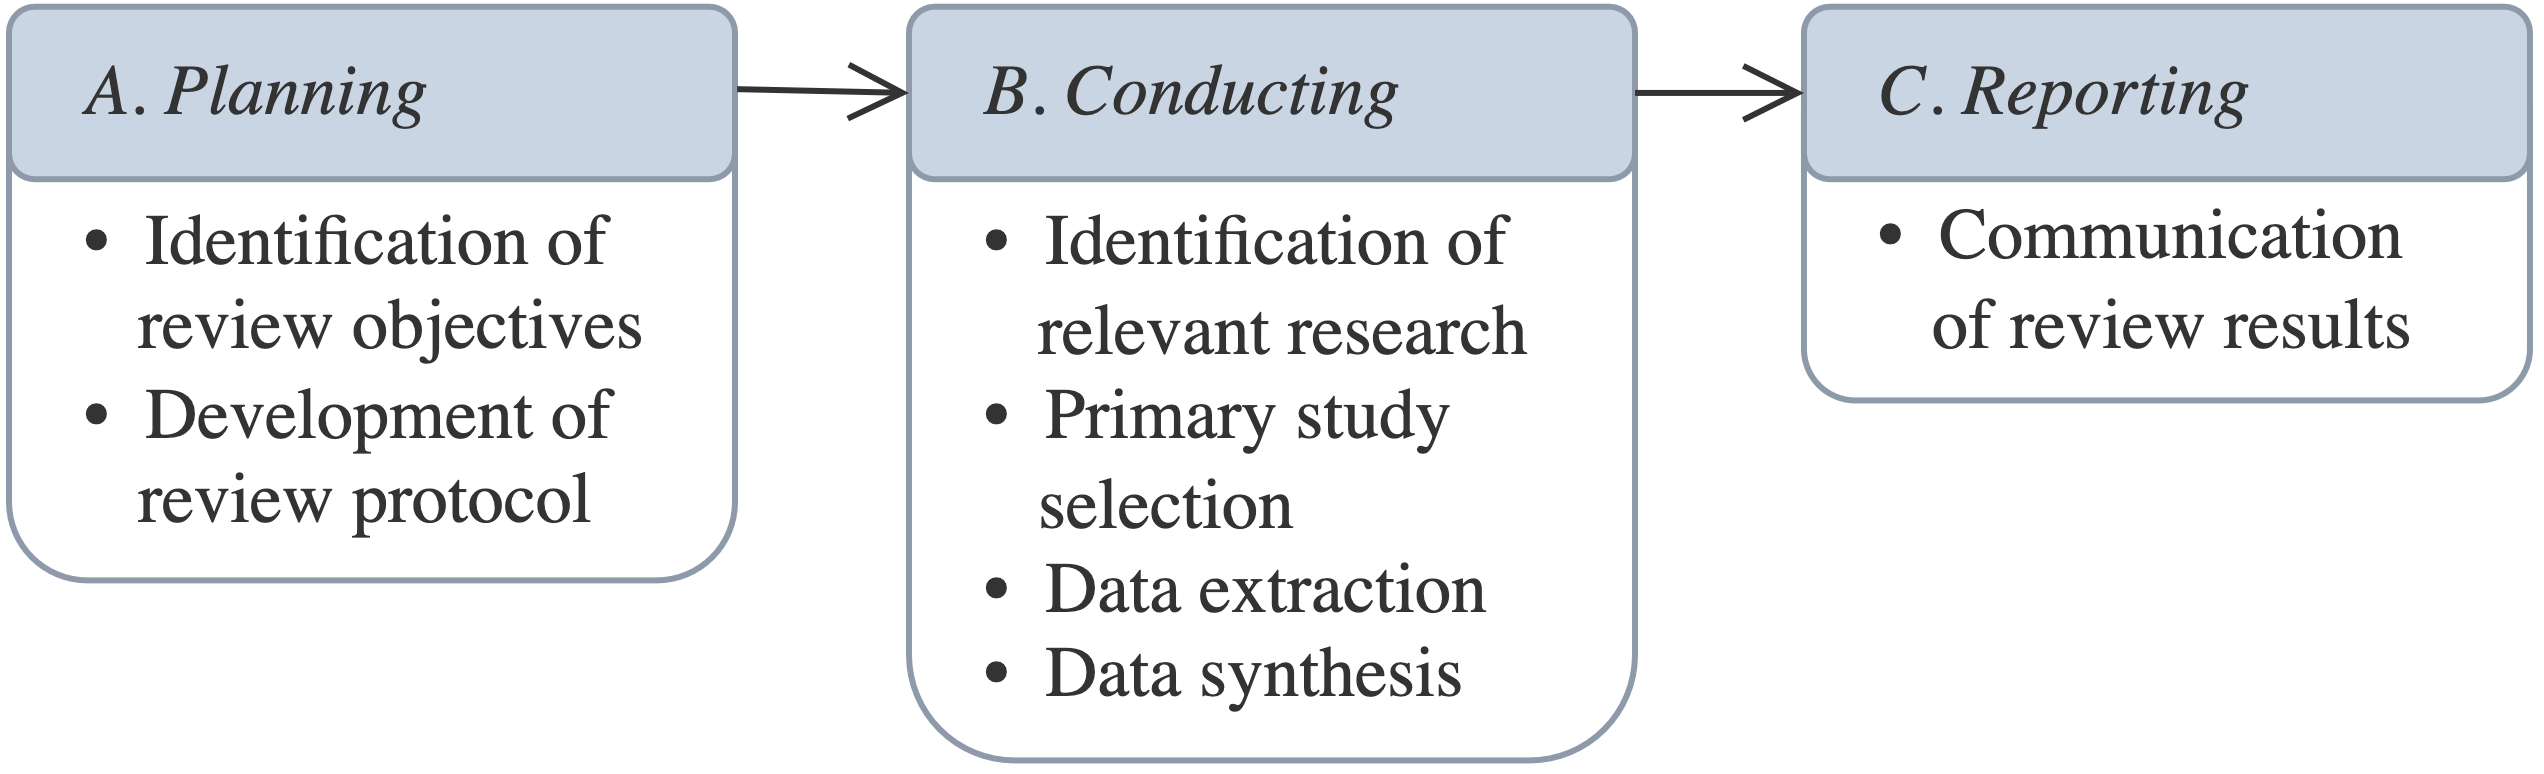
\includegraphics[width=0.489\textwidth]{images/systematic_review_diagram.png}
    \caption{The three phases of a systematic literature review\cite{GuidelinesPerformingSystematic}}
    \label{Fig:slr_diagram}
\end{figure}

\subsection{Planning the review}
\subsubsection{Research questions}
\label{research_questions}

In this sub-section, we aim to address the background, objective, and outcome of conducting the survey.
\begin{itemize}
    \item \textbf{Q1:} {What development friction exist for developers working on systems programming projects, such as the linux kernel}?\\
          {This research question aims to identify the common pain points of developers working on systems programming projects, both in onboarding and day-to-day development.
          }
    \item \textbf{Q2:} {How does Rust's language design effect the cognitive load of developers in systems programming}?\\
          {This research question looks at how the various attributes of the language, such as the concept of ownership, algebraic data types, forced error handling effect
          the cognitive load of developers, both positively and negatively.}
    \item \textbf{Q3:} {How does the workflow (use of tools for common task) differ between the two langauges}?\\
          {In this research question we'll explore how systems programmers accomplish various programming related tasks, such as debugging, testing, and profiling.
          we'll look at what tools are used, their strengths and limitations, and the level of integration each tool has with the development environment}
          % \item \textbf{Q4:} {What were the motivations behind projects that have done a full or partial migration between the two? How did that effect the developer experience}?\\
          % {In this research question we'll look at the motivations behind projects that have migrated from C to Rust, or have adopted Rust for new development. 
          % We'll also explore the current level of interoperability of the two languages, and the outcomes for projects that did a full migration?}
\end{itemize}

\subsubsection{Search Strategy}
\paragraph{\color{Black}Define search terms}{Developer Experience, Cognitive Load, Cyclomatic Complexity, Static Analysis,  linux kernel, embedded, scientific computing, drivers, browser, network, Rust, C}
\paragraph{\color{Black}Digital libraries used} {IEEE Xplore, ACM Digital Library, Google Scholar, Google}
\paragraph{\color{Black}Any issues using search terms}{ \begin{itemize}
        {\item Developer Experience tends to return papers related to the experience level of developers, rather than the experience of developers.}
              {\item it seems difficult to find papers at the intersection of systems programming and developer experience}
              {\item C is a letter, and it seems difficult to limit the results to those related to the programming language if tied to phrases that are used heavily across domains (such as "cognitive load").}
    \end{itemize}
}

\subsubsection{Study selection}
In this sub-section, we aim to define the survey's scope by defining the development areas and the filtering process we followed.

The study selection process is constrained by the inclusion criteria (IC) and exclusion criteria (EC). A paper or source was included if all the following were met:
\begin{itemize}
    \item IC1 The target population of the study, or source, were developers working on relevant projects, such as the linux kernel, or were working in a domain such as embedded systems or scientific computing, where highly constrained resource management is a defining characteristic.
    \item IC2 The langauges involved in those projects were Rust and/or C, or the paper discussed topics relevant to the development in those languages such as tooling, or ecosystem maturity.
    \item IC3 The paper either focused or touched on the developer experience, or related topics such as cognitive load, productivity, or developer velocity
\end{itemize}
A paper will be rejected if any of the following are met:
\begin{itemize}
    \item EC1 The study or source is not in or translatable to english
    \item EC2 If it isn't a paper, the source is neither from a developer working on, nor documentation for, a relevant project.
    \item EC3 The focus of the source is on performance or memory safety in isolation of any relevant impact on developers or the development process
\end{itemize}

\subsubsection{\color{Black} Data extraction and systhesis}
\label{data_collection}
{
    As the sources found seem to touch on different intersections of the research questions, we searched for different combinations of search terms relevant to the topics involved.
    For developer experience we stared with terms like developer experience, developer velocity, and cognitive load, but then moved on to terms like "Cyclomatic Complexity" and "Static Analysis".
    For systems programming, as it is a umbrella for different categories of projects that are often studied
    by themselves, we substituted phrases like "embedded", "linux kernel", and "scientific computing", in an Parenthesized or statement in the search engines that supported it. We also searched for the terms "Rust" and "C" in combination with the other terms, to try and find papers that discussed the two languages in relation to each other.
    We filtered papers generally to those published in the last 5 years, mostly due to it lowering the noise of the results(though unfortunately some older relevant papers may be filtered out). We tended to cycle between using google scholar, and then traditional academic databases.
    While we stared primarily with the academic databases, the
    lack of semantic search tended to increase the amount of papers unrelated to programming, and we then transitioned to primarily using google scholar which is a meta search engine.
    Often we would find a paper that seemed relevant, and then look at the papers it cited, and the papers that cited it.
    When searching for non-academic sources, we used google and outside of pages that we linked only provide definitions for terms used in the paper, we only have one non-academic source, which
    is a blog post by one of the primary contributors to Rust's asynchronous programming model.
}

\subsection{\color{Black} Conducting the review}
\label{conducted_review}
{
    Searching in this manner tended to return a lot of irrelevant results. Developer experience tended to return more results related to the experience level of developers than the experience of development in a given context, and searching for papers related to C and any other search phrase that wasn't exclusive to programming tended to return mostly irrelevant results
    unless the search engine used had some form of vector search(where words are mapped to a vector space, and the distance between the vectors is used to determine similarity). We find that papers exploring rust for some domain related to systems programming generally have some comparison to C, and some discussion of the developer experience, but that the developer experience is rarely the focus of the paper.
    We did find one paper(so far) that seems extremely relevant to the topic where Rust and C were compared for the difficulty of solving a common HPC benchmarking problem and the relative performance of the two implementations. Papers related to development experience tended to be the most relevant, but also the most difficult to find.
}

\subsubsection{\color{Black}List the number of papers retrieved from digital libraries}
{The search was conducted between 2023-09-15 and 2023-11-24, here is the number of papers retrieved from each digital library:}
\begin{itemize}
    \item IEEE Xplore: 5
    \item ACM Digital Library: 7
    \item PeerJ: 2
    \item usenix.org: 1
    \item springerLink: 1
    \item Other: 3
    \item Google: 3
    \item Total: 22
\end{itemize}

Other includes paper found through google scholar but were not hosted on a academic database, such as a thesis, or a paper hosted on a personal website.
google was for non-academic sources, such as blog post or github issues.

\begin{table}[!htbp]
    \caption{List of Papers}
    \label{tab:primary_papers}
    \centering
    \def\arraystretch{1.3}
    \begin{tabular}{p{0.1\linewidth}p{0.65\linewidth}p{0.1\linewidth}}
        \hline
        ID  & Author(s)                            & Ref                                                         \\
        \hline
        \hline
        S1  & Costanzo, Manuel et al.              & \cite{costanzoPerformanceVsProgramming2021}                 \\
        \hline
        S2  & Fakhoury, Sarah et al.               & \cite{fakhouryEffectPoorSource2018}                         \\
        \hline
        S3  & Nadeem, Ayman                        & \cite{nadeemHumancenteredApproachStaticanalysisdriven2022a} \\
        \hline
        S4  & Davis, Gwen                          & \cite{davisDeveloperExperienceWhat2023}                     \\
        \hline
        S5  & Noseda, Mario et al.                 & \cite{nosedaRustSecureIoT2022}                              \\
        \hline
        S6  & Sudwoj, Michal                       & \cite{sudwojRustProgrammingLanguage2020}                    \\
        \hline
        S7  & Fulton, Kelsey R. et al.             & \cite{fultonBenefitsDrawbacksAdopting2021}                  \\
        \hline
        S8  & Astrauskas, Vytautas et al.          & \cite{astrauskasHowProgrammersUse2020}                      \\
        \hline
        S9  & Fagerholm, Fabian et al.             & \cite{fagerholmDeveloperExperienceConcept2012}              \\
        \hline
        S10 & Graziotin, Daniel et al.             & \cite{graziotin2015you}                                     \\
        \hline
        S11 & Gulati, Aryan                        & \cite{gulati2022can}                                        \\
        \hline
        S12 & Hu, Shuang et al.                    & \cite{huComprehensivenessAutomationLifecycle2022}           \\
        \hline
        S13 & Noda, Abi et al.                     & \cite{nodaDevExWhatActually2023}                            \\
        \hline
        S14 & Oikawa                               & \cite{oikawaExperienceDevelopingFAT2023}                    \\
        \hline
        S15 & Developer Experience DevEx           & \cite{DeveloperExperienceDevEx}                             \\
        \hline
        S16 & Saiorse                              & \cite{saoirseWhyAsyncRust2023}                              \\
        \hline
        S17 & Xu, Hui                              & \cite{xuMemorySafetyChallengeConsidered2021}                \\
        \hline
        S18 & Britannica                           & \cite{SystemsProgrammingDefinition}                         \\
        \hline
        S19 & Guidelines for Performing Systematic & \cite{GuidelinesPerformingSystematic}                       \\
        \hline
        S20 & Balasubramanian et al.               & \cite{balasubramanianSystemProgrammingRust2017}             \\
        \hline
        S21 & Rooney, Sean et al.                  & \cite{rooneyEvaluatingFFTPerformance2023}                   \\
        \hline
        S22 & Tracey, Brendan et al.               & \cite{traceyGradingCurveHow2023}                            \\
        \hline
        S23 & Nischal, Shrestha                    & \cite{shresthaHereWeGo2020}                                 \\
        \hline
        S24 & Ardito, Luca et al.                  & \cite{arditoEvaluationRustCode2021}                         \\
        \hline

    \end{tabular}
\end{table}
\subsection{Threats to validity}
{
    The primary threat to validity is the lack of information related to the development experience of C developers. While we have papers which compare rust and c in a specific context, such as embedded systems,
    the focus of those papers is on rust, and they lack information on the development experience of C developers. We have papers which measure indicators of developer experience, such as the cyclomatic complexity
    of a C program, but these approximations only tell us about the complexity of the code. For example there could exist a tool or ide that makes it easier to reason about the code, and is used in professional settings but
    was not mentioned in the papers selected.
}

{
    The second threat to validity is selection or publication bias. The papers selected were selected based on the search terms used, and their relevance to the research questions. The papers which examined rust, while critical of the language, tended
    towards a positive view of the language. It could be that the papers selected are not representative of the general view of the language, or that the papers which are critical of the language were not as discoverable.
}

{
    The third threat to validity is researcher bias. While we attempted to be as objective as possible, since we are familiar with rust and we were not employing a quantitative methodology,
    our familiarity with the language may have influenced our interpretation of the papers selected.
}

\section{Results, Discussion, and Implications}
\label{results}

\subsection{Demographics of the selected studies}
% The demographic subsection provides information about the change in research activity within the scope of the literature survey. This Section should provide the following:
% - Time range of papers in the survey. For example, the articles were published between 2015 and 2023.
% - Activity change that covers the changes in the number of papers produced. This will require making a list 
%   of documents and their publication date. This helps to indicate whether the research area has been gaining attention or not.
{All but 3 Papers selected for this survey were published between 2018 and 2023. two of the outliers were published in 2012\cite{fagerholmDeveloperExperienceConcept2012} and 2015\cite{graziotin2015you} respectively,
    and were included to provide more context on developer experience and how it impacts software development. There was one early paper exploring using rust
    in systems programming\cite{balasubramanianSystemProgrammingRust2017} published in 2017.
    Not counting the guidelines for performing a systematic literature review\cite{GuidelinesPerformingSystematic}, there were
    7 conference papers, 6 journal articles, 1 book entry, 4 web page/blog posts, and 1 thesis. Those which were
    examining rust tended to be more recent, with the oldest being published in 2020\cite{sudwojRustProgrammingLanguage2020}. The only blog post that was posted by
    an individual was \cite{saoirseWhyAsyncRust2023}, and was included as it was created by a contributor to the rust project (and more specifically to the very feature it was discussing).

    only a few of the papers selected were published prior to 2020, with the oldest being a paper on developer experience published in 2012\cite{fagerholmDeveloperExperienceConcept2012}.\\

    %6 conference papers, 6 journal articles, 1 book entry, 4 web page/blog posts, 1 thesis
    \startchronology[startyear=2012,stopyear=2020,height=1pt,  startdate=true, stopdate=true, arrow=false, width=\hsize, box=false]
    \chronoevent[date=false]{06/2012}{\cite{fagerholmDeveloperExperienceConcept2012}}
    \chronoevent[date=false]{2015}{\cite{graziotin2015you}}
    \chronoevent[date=false]{2017}{\cite{balasubramanianSystemProgrammingRust2017}}
    \chronoevent[date=false]{05/2018}{\cite{fakhouryEffectPoorSource2018}}
    \stopchronology

    The majority of the papers were published between 2020 and 2023 inclusively.

    % % Draw the timeline
    \startchronology[startyear=2020,stopyear=2024,height=1pt,  startdate=true, stopdate=true, arrow=false, width=\hsize, box=false]
    \chronoevent[date=false,markdepth=55pt]{2021}{\cite{fultonBenefitsDrawbacksAdopting2021}}
    \chronoevent[date=false,markdepth=55pt]{02/26/2021}{\cite{arditoEvaluationRustCode2021}}
    \chronoevent[date=false,markdepth=55pt]{06/2022}{\cite{nosedaRustSecureIoT2022}}

    \chronoevent[date=false,markdepth=40pt]{11/13/2020}{\cite{astrauskasHowProgrammersUse2020}}
    \chronoevent[date=false,markdepth=40pt]{03/2022}{\cite{nadeemHumancenteredApproachStaticanalysisdriven2022a}}
    \chronoevent[date=false,markdepth=40pt]{2023}{\cite{oikawaExperienceDevelopingFAT2023}}
    \chronoevent[date=false,markdepth=40pt]{10/2023}{\cite{saoirseWhyAsyncRust2023}}

    \chronoevent[date=false,markdepth=25pt]{09/11/2020}{\cite{sudwojRustProgrammingLanguage2020}}
    \chronoevent[date=false,markdepth=25pt]{2022}{\cite{gulati2022can}}
    \chronoevent[date=false,markdepth=25pt]{2023}{\cite{davisDeveloperExperienceWhat2023}}
    \chronoevent[date=false,markdepth=25pt]{03/2023}{\cite{rooneyEvaluatingFFTPerformance2023}}
    \chronoevent[date=false,markdepth=25pt]{06/08/2023}{\cite{nodaDevExWhatActually2023}}

    \chronoevent[date=false]{06/27/2020}{\cite{shresthaHereWeGo2020}}
    \chronoevent[date=false]{09/28/2021}{\cite{xuMemorySafetyChallengeConsidered2021}}
    \chronoevent[date=false,]{10/2021}{\cite{costanzoPerformanceVsProgramming2021}}
    \chronoevent[date=false]{12/2022}{\cite{huComprehensivenessAutomationLifecycle2022}}
    \chronoevent[date=false]{10/2023}{\cite{traceyGradingCurveHow2023}}

    % \chronoevent{2023}{\cite{DeveloperExperienceDevEx}}
    % \chronoevent{2023}{\cite{SystemsProgrammingDefinition}}
    % \chronoevent{2023}{\cite{GuidelinesPerformingSystematic}}

    \stopchronology
    % \begin{tikzpicture}
    %     % Draw horizontal line
    %     \node[anchor=west, text width=6cm] at (0,1.1) {Majority of papers published between 2018 and 2023};
    %     \draw[align=right, line width=1pt] (0,0) -- (8,0);

    %     % Draw vertical lines and labels
    %     \foreach \x/\year in {.5/2012, 1.5/2015, 4.5/2018, 8/2023}
    %         {
    %             \draw (\x,-0.2) -- (\x,0.2);
    %             \node[below] at (\x,-0.2) {\year};
    %         }

    %     % Add labels for the papers
    %     \node[anchor=west] at (0,0.5) {\cite{fagerholmDeveloperExperienceConcept2012}};
    %     \node[anchor=west] at (1.5,0.5) {\cite{graziotin2015you}};

    %     \node[anchor=west] at (7,0.5) {\cite{costanzoPerformanceVsProgramming2021}};
    %     \node[anchor=west] at (4.5,0.5) {\cite{fakhouryEffectPoorSource2018}};
    %     \node[anchor=west] at (7.5,.5) {\cite{nadeemHumancenteredApproachStaticanalysisdriven2022}};
    %     % TODO: Add the rest of the papers
    % \end{tikzpicture}
}

\subsection{Developer Friction in Systems Programming (RQ1)}
{
    This is by far the least covered question currently.Part of the reason for lack of coverage is likely a combination of the focus of research in systems programming,
    and a limitation of the search terms used. Most results related to c and developer experience, or c projects and developer experience, tended to be related to the experience level of developers, and it was difficult to omit terms related to experience level without omitting relevant results, as the developers contacted during
    studies are often either students or senior developers. Another factor was that the papers that compared rust and c
    in a specific context (such as embedded systems\cite{nosedaRustSecureIoT2022}) tended to focus more on rust
    and it's advantages and disadvantages in that context, rather than workflow or tooling used for c development. However, despite the lack of emphasis on C, a few things can be
    derived.
}
{
    First, from the paper on rust in embedded systems\cite{nosedaRustSecureIoT2022}, the authors talked about the utility of user defined types in ensuring correct order of initialization of the gpio output pin and the UART driver.In their words, "Encoding the pin state like this ensures that misconfiguration (or simply forgetting to initialize) is an issue of the past". There is a stringent requirement on ensuring correctness, and a requires a degree of understanding of the underlying physical system. For embedded systems, C's manual memory management and weak typing can be a benefit, as it allows for more direct control over the hardware. However, this sets the bar for entry higher, as
    this puts the requirement for ensuring correctness solely on the developer. In that same paper, the authors also mentioned the use of a static analysis tool for C, and the type of memory bugs they can detect, while also mentioning their limitation. Static analysis tools work well so long as the source code being analyzed is available, which is not the case for dependencies.
}

{
    There is research comparing the likelyhood of new contributors to introduce bugs on their first contribution in rust and C++
    in the Mozilla project, where the rust code was replacing C++ code, and thus a direct comparison could be made.\cite{traceyGradingCurveHow2023}. In this paper, the authors discuss the difficulty in attracting new contributors to existing projects, and how efforts to do so by Mozilla's open source initiatives often stirs anxiety in existing maintainers. The first time contributors often inexperienced, and often existing maintainers don't have the infrastructure to support them. Often they introduce bugs, and the majority of them don't contribute again.
}

{
    Lastly, due to manual memory management, and lack of abstraction, it is difficult to use a language like C in domains like HPC and scientific computing to create software that is both scalable and maintainable\cite{costanzoPerformanceVsProgramming2021}.
}
% Touched on by secure IOT, maybe can rust replace c and the hpc paper

\subsection{How does Rust's language design effect the cognitive load of developers in systems programming? (RQ2)}
{
    In \cite{fultonBenefitsDrawbacksAdopting2021}, most of the
    participants in the survey found rust more difficult to learn than other languages. The concept users
    struggled with the most when initially learning rust was ownership which, given the relative novelty of ownership
    in programming languages, is unsurprising. In \cite{shresthaHereWeGo2020}, the authors discussed the factors that make new programming languages more difficult to learn, and two of the factors where participants mentioned rust explicitly is when the language concept either requires a mindshift or doesn't map to something they already know. Other thinks which contribute to the initial learning curve is that is expression based, and borrows heavily from functional programming.
    % Also, speaking from experience, their are certain patterns that are common in object oriented programming that new developers tend to try to use in rust, like grouping data together 
}
% {
%     There is a tradeoff in rust between the initial learning curve and cognitive load of practiced rust developers.   The learning curve is also impacted by the fact that rust explicitly
%     doesn't use inheritance and (speaking from experience), the tendency to try to use object oriented programming patterns
%     such as wrapping all data in a struct makes for a difficult transition. In that example, the reason is that if you have a
%     function where only some data needs to be mutable, you have to either make the entire struct mutable(which means borrowing it exclusively), or
%     use interior mutability, which can quickly become a complicated endeavor.
% }

{
    The tradeoff is that once you've learned the language, and have reached the point where you're comfortable with it,
    the guarantees provided by the language and the compiler make it easier to reason about the code, and provide a degree
    of confidence that the code will behave as expected. This is in part due to the ability to use the type system to
    enforce invariants, which moves what would otherwise be runtime errors to compile time errors\cite{nosedaRustSecureIoT2022}.
    In \cite{balasubramanianSystemProgrammingRust2017}, the author brings up the utility of rust's properties (which he incorrectly describes as a linear type system rather than affine), and uses this to implement a Software Fault Isolation (SFI) system, and argues
    that rust enables SFI with lower overhead than "any mainstream language". The premise being that since each component only has access to objects granted to it by the allocator or other components, it could be imlemented without copying
}

{
    This does seem to effect how much users trust their code. In \cite{fultonBenefitsDrawbacksAdopting2021}, 90\% of the interview participants slightly or strongly agreed witht he sentiment that their production code was bug free. While for the interview
    portion there was a small sample size and the participants were self selected, that degree of trust does seem to be
    backed up by the data. In\cite{xuMemorySafetyChallengeConsidered2021}, all of the 186 memory safety bugs examined required
    unsafe code. Many of the CVEs were mild soundness issues that open the possibility of undefined behaviour in safe rust.
}

{
    a quick note about soundness. Rust has a concept of soundness, which is the guarantee that if the code is written in 100\% safe rust cannot have undefined behavior. To say that a library or application is sound means that all possible uses of the it cannot lead to undefined behavior.
    The program will execute in a predictable, deterministic manner. These are guarentees that the community takes seriously, and often violations of soundness are (arguably misguidedly) reported and treated as vulnerabilities\cite{xuMemorySafetyChallengeConsidered2021}\cite{traceyGradingCurveHow2023}.
    These vulnerabilities would not exist in C or C++, simply because they make no such guarantees.
}

{
    When comparing the likelyhood of new contributors to introduce vulnerabilities in rust and C++ in the Mozilla project, the author found that first time rust contributors were 70 times less likely to introduce a vulnerabilty.
    Many of the vulnerabilities in the rust code were soundness issues, and all required unsafe code\cite{traceyGradingCurveHow2023}. It's worth noting that, as pointed out by a few people in the cpp subreddit,
    the comparison was not entirely fair, and the multiple of 70 is likely an overestimate. On the first point, the rust code was replacing C++ code, and thus some of the contributors likely referenced the module they
    were replacing. On the second point, looking at the data on commits and vulnerabilities listed in the study itself leads to a much more conservative interpretation (5x or 6.5x).
}

%TODO: add paragraph for how users are using unsafe

{
    As far as the inherent complexity of the language, rust is seems to sit between c, c++ and higher languages. In \cite{arditoEvaluationRustCode2021}, Rust was compared to a set of other languages (including C) in terms of cyclomatic complexity, halstead metrics, and cognitive complexity, and Maintainability Index. These metrics are all related to the cognitive load of developers. Cyclomatic complexity measures the number of linearly independent paths through a program, and provides a rough estimate of how difficult it is to test and modify. Halstead metrics are a set of metrics that approximate software properties such as the length(the number of operators and operands),volume(information content of a program),and time it would take a programmer to implement, to name a few. Cognitive complexity is a measure of how difficult it is to intuitively understand a piece of code and is based on the sum of the cognitive weights of basic softare control structures. The maintainability index is a composite metric that attempts to approximate the maintainability of a piece of software. In all the metrics, rust outperformed C (and C++), though it's worth mentioning that in all except cognitive complexity it performed worse than higher level languages. It had the lowest cognitive complexity of all the languages tested.
}

{
    In\cite{nodaDevExWhatActually2023}, the authors stated that one of the primary factors in developer experience is
    the length of feedback loops. One of the areas that rust is lacking in is compile time, and for larger projects, especially those
    which make heavy use of macros, generics, and user defined types, compile times can be a significant issue. Part of the issue is that
    the rustc frontend is single threaded, though there is work being done to address this \cite{TrackingIssueParallel}.
}

\subsection{Differences in Workflow (RQ3)}
{
    %in rust heavy use of static analysis, and cargo as the goto tool for everything
    To a certain extent this, like the findings for RQ1, is difficult to answer for C without drawing on personal experience. The papers that
    compared the two languages mentioned tools and workflow information for C in passing. In \cite{nosedaRustSecureIoT2022},
    the authors mentioned a series of static analysis tools for C and what type of (memory safety) issues they could be
    used to detect. In \cite{costanzoPerformanceVsProgramming2021} the authors briefly layed out the C implementation, it's use
    of openMP, and the directives used for things like SIMD operation. In \cite{saoirseWhyAsyncRust2023}, the author talked about how userspace
    concurrency is handled in C: "People implementing highly performant network services in languages without facilities for user-space
    concurrency like C tend to implement them using a hand-written state machine."
}

{
    Given the (current) lack of information on the workflow for C, I can only make broad assumptions about
    the general process of developing in C. First, since there is no package manager, a few large libraries
    are used almost universally for some tasks, such as openMP. Most things are implemented from scratch as needed.
    Static analysis tools exists, but they play a smaller role in the development process. Third, writing code is easier,
    but it requires a more is left to the developer to ensure correctness. Lastly, there are tools for most tasks, but developers (or teams) are partially
    rolling their own tooling.
}

{
    In rust, due to cargo's function as a package manager and tool for publishing packages (called crates),
    there is more of a focus on code reuse. There are currently 132,254 published crates, and while a large
    portion of those are either small utilities or are no longer maintained, there is a crate for most tasks.
    Because Cargo is also how you  generate documentation and publication automatically generates
    documentation from the public API, documentation is up to date and in at least a basic form for all crates.
    Each crate links to a repository, and an entry on doc.rs, which is a site that hosts documentation for crates,
    it also contains the source for that specific published version of the crate.
}

{
    %in rust heavy use of static analysis, and cargo as the goto tool for everything
    Static analysis is built into the compiler, it is how ownership and lifetimes are enforced, and violations of those
    rules can be detected without compiling via cargo clippy, which can be called by the language server rust-analyzer.
    This makes compilation less prominent in the development process.
}

% \subsection{Motivations for Migration(RQ4)}
% {\color{OrangeRed} \lipsum[1-2]}

\section{Conclusion}
 {
  There are areas where rust is lacking: it's ecosystem varies in maturity, and it's compile times can be bad under the right circumstances.
  It's definitely hard to learn if you are comparing it to either c or c++, or anything else that isn't haskell.
  However, it's also a language that is designed to be difficult to use incorrectly, and one that by some metrics is fairly easy to reason about.
  It's a language that, once learned, provides an ergonomic set of tradeoffs that helps developers write code that is both correct and performant.
 }

 {
  Their is an inherent difficulty in the tasks relevant to the domain: writing device drivers, managing an OS, or writing a browser that both connects and protects users from the internet.
  C has been the goto language for these tasks for decades and unfortunately, that is unlikely to change (soon).
  It's fast, and in experienced hands it's memory safety issues can be mitigated, but if all it took to write correct code was experience, we wouldn't have the bugs we have today.
 }

 {
  In some ways, this isn't a fair comparison. Rust was built to address the issues and frustrations that developers had with C++, which had an origin not too different in regards to C.
  I strongly suspect that the reason why the community is so focused on defacto standards and one single build tool that does most things is because how fragmented the C++ ecosystem is.
  Drawing on personal experience, it has some of the best error messages out of any language I've used, and the level of integration between the language and the tooling means I spend
  less time on the meta tasks of development such as configuring my editor or build system, and more time on the actual task at hand.
 }

 {
  One of the things mentioned in \cite{traceyGradingCurveHow2023} is how the risk of introducing vulnerabilities limits open source projects ability to attract and support new contributors.
  Rust provides a way to mitigate that risk, and leverage the type system to both communicate relationships between components and enforce them.
  There is a victory in knowing, at the very least, that PR you just merged from some well intentioned stranger of questionable competence won't cause an explosion.
 }

\subsection{Future Work}
{
There were a few questions I had but were not addressed in the papers I found. The First is how rust compares to c (and c++) when using \texttt{\#![no\_std]}, which is a crate attribute that causes the
compiler to not link to the standard library. It is used in embedded systems, or when the amount of space available is limited. I'm curious how the lack of a standard library effects
the development process. The second is if there is some measure of information density per line or expression, how would rust compare to other languages? between the type system, lifetime
annotation, and the explicit mutability, I'm curious how much information is conveyed per line of code. The third is for programs where there are variants in Rust and C, how complex is the
implementation? This, again, draws perhaps too much from personal observation, but I've noticed a tendency of rust developers to do things like attempt to eliminate clones (method for deep copying),
among other attempts to reduce the amount of memory allocated. I'm curious whether this `tendency' is actually something that is common, and how much of an impact it has on the complexity of
a rust program compared to it's C counterpart.
}

% Comment out nocite once references are cited.        
%\nocite{*}
\bibliographystyle{unsrt}
\bibliography{references}

\end{document}
